% !TeX spellcheck = de_DE/GB


\chapter{Beschreibung der Software IDE}

\section{Installation der Arduino IDE}
Um Mikrocontroller von Arduino, wie den verwendeten Arduino Nano 33 BLE Sense Lite, programmieren zu können, wird die Software namens Arduino IDE in der Version 2.3.2 verwendet. 
Alternativ dazu könnten auch andere Entwicklungsumgebungen, wie Qt verwendet werden, die eine Programmierung in der Programmiersprache C++ ermöglicht.
Vorteil der Arduino IDE sind vor allem ihre Funktionen, die das Einbinden der Software auf dem Mikrocontroller vereinfachen.
Der Bezug der Software Arduino IDE erfolgt über die offizielle Webseite von Arduino, welche unter \url{www.arduino.cc/software} erreichbar ist. Auf dieser Plattform stehen diverse Versionen, für unterschiedliche Betriebssysteme, wie Windows, Linux und Mac OS X, sowie in verschiedenen Dateiformaten, zur Auswahl bereit \cite{Arduino.2024}. Um die Anwendung zu installieren, muss die heruntergeladene Datei ausgeführt und den Installationsanweisungen gefolgt werden. Danach ist die korrekte Konfiguration des verwendeten Entwicklungsboards sowie die Installation entsprechender Bibliotheken erforderlich.

\section{Beschreibung der Entwicklungsumgebung}
Nach dem Start der installierten Anwendung öffnet sich die Hauptoberfläche.
\begin{figure}[htb]
	\begin{center}
		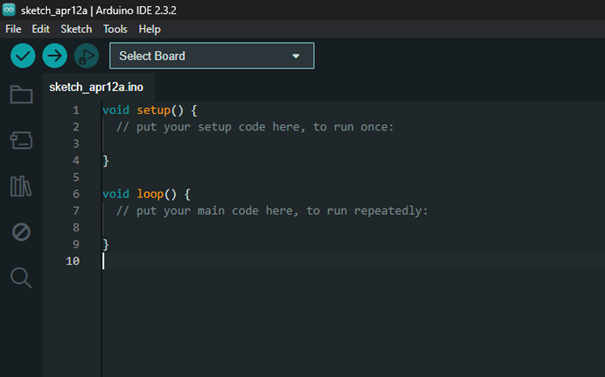
\includegraphics[width=\textwidth]{General/HauptoberflaecheIDE.png}
		\caption{Hauptoberfläche in der Arduino IDE} \label{Hauptoberfläche in der Arduino IDE}
	\end{center}
\end{figure}
Oben in der Hauptoberfläche befindet sich eine Menüleiste, die verschiedene Menüs wie \textit{Datei}, \textit{Bearbeiten} und \textit{Sketch} enthält. Diese Menüs ermöglichen das Bearbeiten und Öffnen von Sketches, also Programmen in der IDE, das Kompilieren und Hochladen von Code sowie das Verwalten von Bibliotheken. Außerdem bietet die Menüleiste ein Hilfe-Menü, das bei Fragen und Problemen hilfreich ist. 
Die Symbolleiste auf der linken Seite der Hauptoberfläche bietet Schaltflächen für häufig genutzte Funktionen wie das Verwalten von Sketches, Boards und Bibliotheken.
Im Zentrum der Hauptoberfläche befindet sich ein Code-Editor, der die Bearbeitung der Sketches ermöglicht. Direkt darunter erscheint nach dem ersten Kompilieren eines Sketches ein Ausgabefenster, das den Kompilierungs- und Hochladeprozess sowie eventuelle Fehler während der Kompilierung anzeigt. Dadurch können Probleme im Code schnell identifiziert werden.

\section{Erste Schritte in der Entwicklungsumgebung}
\subsection{Auswahl des Mikrocontrollers}
In der Entwicklungsumgebung können sofort Sketche geöffnet und geschrieben werden. Um den Sketch aber kompilieren zu können, muss das korrekte Board ausgewählt werden.
Dafür muss zunächst das passende Board installiert werden. 
 Dies erfolgt über den \textit{Boards-Manager}.
\begin{figure}[htb]
	\begin{center}
		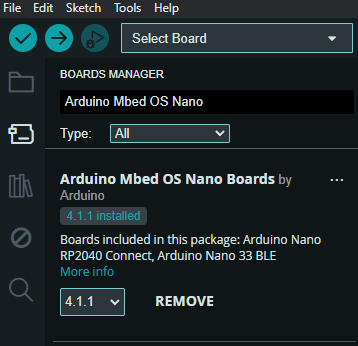
\includegraphics[width=\textwidth]{General/Boardsmanager}
		\caption{Installation des Boards} \label{Installation des Boards}
	\end{center}
\end{figure}
Im \textit{Boards Manager} kann in diesem Fall die Datei Arduino Mbed OS Nano in der aktuellen Version 4.1.1 heruntergeladen und installiert werden. Danach kann unter \textit{Select Board} das Board Arduino BLE Sense 33 ausgewählt werden \cite{Arduino.2024b}.
Alternativ kann das Board über ein USB-Kabel angeschlossen werden. Unter\textit{ Select Board} wird bereits das korrekte Board und der entsprechende COM, also in diesem Fall der USB-Port, angeboten. Werden diese ausgewählt, sind die Installationsanweisungen zu befolgen, um das Board zu installieren.

\subsection{Bibliotheken einbinden}
Von Arduino gibt es bereits sehr viele offiziell unterstützte Bibliotheken. Will man diese in einem Sketch nutzen, muss man diese zunächst installieren.
Dafür kann über den \textit{Library Manager} die nötige Bibliothek heruntergeladen und installiert werden. Die Suchfunktion hilft dabei, die korrekte Bibliothek zu finden \cite{Arduino.2024c}.
\begin{figure}
	\begin{center}
		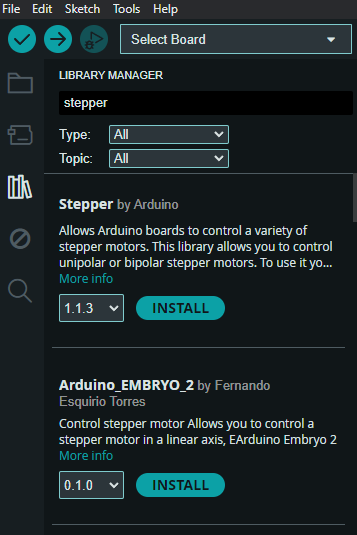
\includegraphics[width=\textwidth]{General/Librarymanager}
		\caption{Herunterladen von Bibliotheken} \label{Herunterladen von Bibliotheken}
	\end{center}
\end{figure}
Nachdem die Bibliothek installiert ist, kann sie im header in den Sketch eingebunden werden.
Bei Verwendung von Bibliotheken, die nicht im \textit{Library Manager} zu finden ist, kann diese über \textit{Sketch->Include Libraries->Add .ZIP Library…} eingebunden werden.

\section{Programmierung}
Wird ein neuer Sketch geöffnet, sind bereits die Funktionen \textit{void setup()} und \textit{void loop()} hinterlegt.

\subsection{header}
Im \textit{header} werden vor allem alle nötigen Bibliotheken hinterlegt und initialisiert. Gleichzeitig können hier aber auch Adressen von Peripheriegeräten hinterlegt und erste wichtige Variablen definiert werden.

\subsection{setup()}
Die \textit{void setup()}-Funktion wird bei jedem Neustart oder Reset einmal ausgeführt \cite{Arduino.2024d}.
Hier wird zum Beispiel die serielle Kommunikation gestartet, aber auch verwendete Pins initialisiert und zugewiesen.

\subsection{loop()}
In der \textit{void loop()}-Funktion findet der größte Teil des Programms statt. Der Inhalt dieser Funktion wird dauerhaft wiederholt, bis entweder kein Strom mehr an dem Arduino anliegt, oder der Reset-Knopf gedrückt wird und somit zunächst erst die \textit{void setup()}-Funktion wieder gestartet wird \cite{Arduino.2024e}.

\section{Erster Programmtest}
Um die Funktion eines Systems zu testen, wird oft zunächst ein sehr simples Programm oder eine sehr grundlegende Funktion getestet.
In diesem Fall kann hier über \textit{Datei -> Beispiele -> 01.Basics -> Blink} ein Sketch geöffnet werden, in dem die auf dem Arduino Nano 33 BLE Sense Lite aufgebrachte LED in einem fest gelegten Takt blinkt, wodurch die korrekte Auswahl des Boards und die Übertragung des Sketches auf den Mikrocontroller getestet werden können.

\begin{lstlisting}
void setup() {
	pinMode(LED_BUILTIN, OUTPUT);
}
void loop() {
	digitalWrite(LED_BUILTIN, HIGH);
	delay(1000);                     
	digitalWrite(LED_BUILTIN, LOW);  
	delay(1000);                     
}
\end{lstlisting}

In der \textit{void setup()}-Funktion wird in diesem Beispiel über den Ausdruck \textit{pinMode(LED BUILTIN, OUTPUT)} die auf dem Mikrocontroller verbaute LED in dem Sketch aufgerufen und eingebunden.
In \textit{void loop()} wird durch den Befehl\textit{ digitalWrite()} die LED eingeschaltet, indem eine Spannung an sie angelegt wird. Nach einer kurzen Verzögerung durch den gleichen Befehl wird die LED dann wieder ausgeschaltet, indem die anliegende Spannung gesenkt wird. Die Verzögerung kann mit dem \textit{delay()}-Befehl eingestellt werden, indem der Wert in der Klammer angepasst wird. Dabei wird der Wert in Millisekunden angegeben.
